\documentclass[serif,xcolor=pdftex,dvipsnames,table,hyperref={bookmarks=false,breaklinks}]{beamer}

%%%%%%%%%%%%%%%%
% Change the macros below to configure the title slides
% for your course.
\newcommand{\coursename}{COMPSCI 590N}
\newcommand{\instructor}{Roy J. Adams}
\newcommand{\university}{University of Massachusetts Amherst}
\newcommand{\department}{College of Information and Computer Sciences}
%%%%%%%%%%%%%%%%

\newcommand\HUGE{\@setfontsize\Huge{50}{60}}

\newcommand{\settitlecard}[2]{
  \title[\coursename  Lecture #1] 
    {\coursename \\ Lecture #1: #2}
     \author[\instructor]{\instructor}
     \institute[\university]{
     \department\\
     \university
   }
\date{}
}

\newcommand{\maketitlepage}{
  \begin{frame}
  \titlepage
  %\center{
    %If you use the slides unmodified, retain the attribution below
  %  \tiny{Slides by Roy J. Adams (rjadams@cs.umass.edu). 
    %If you modify the slides, please retain the alternate attribution below
    %\tiny{Based on slides by Roy J. Adams (rjadams@cs.umass.edu). \\    
  %  }                                              
  %}  
  \end{frame}
}

\AtBeginSection[]
{
  \begin{frame}<beamer>{Outline}
    \tableofcontents[currentsection,subsectionstyle=hide]
  \end{frame}
}


\newcommand{\cut}[1]{}

\newcommand{\iconbox}[4]{
  \only<#1-#2>{
    \begin{columns}[T]
      \column{0.5in}
           \includegraphics[width=0.5in]{#3}
       \column{3.7in}
            #4
    \end{columns}
    \medskip
    \medskip
    \medskip
  }
}

\mode<presentation>{
  \usepackage{../beamertheme589theme}
  \setbeamercovered{invisible}
}

\mode<handout>{
  \usepackage{../beamertheme589theme}
  \setbeamercovered{transparent}
}


\usepackage[english]{babel}
\usepackage[latin1]{inputenc}
\usepackage{times}
\usepackage[T1]{fontenc}
\usepackage{amsmath}
\usepackage{amssymb}
\usepackage[noend]{algorithmic}
\usepackage{algorithm}
\usepackage{listings}
\usepackage{tcolorbox}
\usepackage{xmpmulti}

\renewcommand\mathfamilydefault{\rmdefault}

\newcommand{\setA}{\mathcal{A}}
\newcommand{\setB}{\mathcal{B}}
\newcommand{\setS}{\mathcal{S}}
\newcommand{\setV}{\mathcal{V}}
\DeclareMathOperator*{\union}{\bigcup}
\DeclareMathOperator*{\intersection}{\bigcap}
\DeclareMathOperator*{\Val}{Val}
\newcommand{\mbf}[1]{{\mathbf{#1}}}
\DeclareMathOperator*{\argmax}{arg\,max}
\DeclareMathOperator*{\argmin}{arg\,min}
\DeclareMathOperator*{\sign}{sign}
\newcommand{\deriv}[2]{\frac{\partial{#1}}{\partial{#2}}}

\lstdefinestyle{custompython}{
  belowcaptionskip=1\baselineskip,
  breaklines=true,
  frame=single,
  xleftmargin=\parindent,
  language=Python,
  showstringspaces=false,
  basicstyle=\footnotesize\ttfamily,
  keywordstyle=\bfseries\color{green!40!black},
  commentstyle=\itshape\color{purple!40!black},
  identifierstyle=\color{blue},
  stringstyle=\color{orange},
}
\lstset{style=custompython}

\makeatletter
\renewcommand*\env@matrix[1][*\c@MaxMatrixCols c]{%
  \hskip -\arraycolsep
  \let\@ifnextchar\new@ifnextchar
  \array{#1}}
\makeatother

\newcommand\norm[1]{\left\lVert#1\right\rVert}


\settitlecard{4}{Computing Special Functions}

\begin{document}

\maketitlepage

\section{Preliminaries}
\subsection{Foo}


% \begin{frame}[t]{Announcements}
% 	\begin{itemize}[<+->]
% 		\item Quiz 2 due tonight.
% 		\item Assignment 2 will be released tomorrow and due next Thursday.
% 		\begin{itemize}[<+->]
% 			\item \textbf{Be sure to run your code.}
% 		\end{itemize}
% 	\end{itemize}
% \end{frame}

\begin{frame}[t,fragile]{Miscellaneous Python Stuff}
	\begin{itemize}[<+->]
		\item \textbf{Comments} allow you to write notes about your code.
	\end{itemize}
	\pause
	\begin{tcolorbox}
		\begin{verbatim}
			# Single line comment
			
			"""
			Multi-line
			Comment
			"""
		\end{verbatim}
	\end{tcolorbox}
	\pause
	\begin{itemize}[<+->]
		\item Mixing tabs and spaces when indenting code will cause an error.
	\end{itemize}
\end{frame}

\section{Computing Special Functions}
\subsection{Foo}

\begin{frame}[t]{Numerical Algorithms}
	\begin{itemize}[<+->]		
		\item So far we discussed how numbers are represented in a computer and how these representations can result in errors
		\item In numerical computing we must also manipulate numbers, which can introduce further errors. 
		\item \textbf{Numerical algorithms} approximate mathematical functions under the restriction of finite precision and finite time.
	\end{itemize}
\end{frame}

\begin{frame}[t]{Long Division}
	\centering
    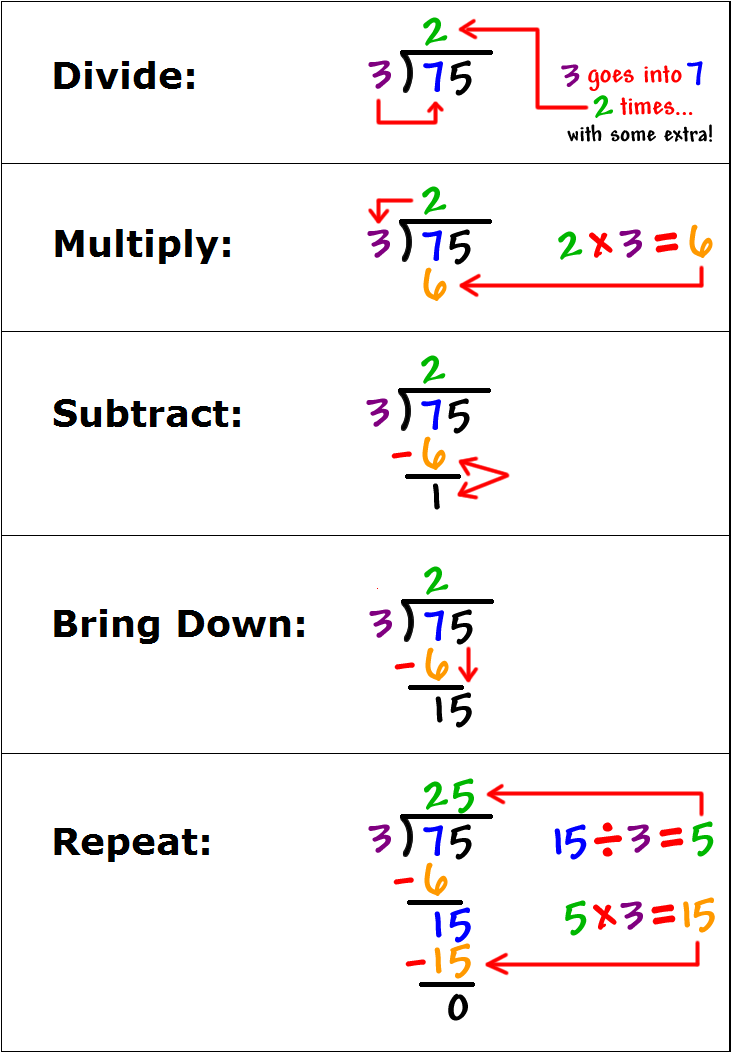
\includegraphics[height=2.5in]{{../Figures/long_division}.png}
\end{frame}
	
\begin{frame}[t]{Types of Numerical Algorithms}
	\begin{itemize}[<+->]
		\item Generally, numerical methods fall into one of two categories:
	\end{itemize}
	
	\pause
	\begin{block}{Direct}
		A direct method is guaranteed to terminate in a finite number of steps and would return the exact answer if we had infinite precision.
	\end{block}
	
	\pause
	\begin{block}{Iterative}
		An iterative method is never guaranteed to terminate, but instead builds a sequence of increasingly accurate approximations and terminates when a desired accuracy is achieved.
	\end{block}
	
\end{frame}

\begin{frame}{Numerical Algorithms}
	\begin{itemize}[<+->]
		\item We have already seen how errors can be caused by rounding. 
		\item Rounding can affect numerical methods in different ways.
		\item Two algorithms that should mathematically give the same result can behave very differently when confronted with the errors caused by finite precision.
	\end{itemize}
	
	\pause
	\centering
	\Huge{DEMO}
\end{frame}

\begin{frame}[t]{Numerical Algorithms}
	The main notion of how well a numerical algorithm performs is called \textbf{stability}:
	
	\pause
	\begin{block}{Stability}
		A numerical algorithm is said to be \textbf{stable} if small errors, no matter what their source is, do not cause large errors in the final result.
	\end{block}
	
	\pause
	\begin{itemize}[<+->]
		\item Examples:
		\begin{enumerate}[<+->]
			\item If an algorithm allows representability errors to accumulate through addition, then we would call this algorithm unstable.
			\item Most iterative algorithms start with an initial guess and refine it. If the accuracy of a method is highly sensitive to the initial guess, then we would call this method unstable.
		\end{enumerate}
	\end{itemize}

\end{frame}
	
	

\begin{frame}[t]{Special Functions}
	\begin{itemize}[<+->]
		\item Unfortunately, most of the standard mathematical functions we use cannot be computed directly and so must be approximated using numerical methods.
		\item Examples: square root, logarithm, exponentiation, and sine/cosine
		\item While you will likely never need to implement these algorithms (most are implemented in hardware!), it is important to know how they are implemented as it can have a large impact on the speed of your programs.
		\item In the following slides we will talk about some general techniques for approximating these functions and then look at a few examples.
	\end{itemize}
\end{frame}

\begin{frame}[t]{Bit-by-bit Methods}
	\pause
	\Huge
	\vspace{1cm}
	\centering
	\begin{tabular}{c c c c}
		1 & 3 & 5 & 7\\
		9 & 11 & 13 & 15\\
		17 & 19 & 21 & 23\\
		25 & 27 & 29 & 31\\
	\end{tabular}
\end{frame}

\begin{frame}[t]{Bit-by-bit Methods}
	\Huge
	\vspace{1cm}
	\centering
	\begin{tabular}{c c c c}
		2 & 3 & 6 & 7\\
		10 & 11 & 14 & 15\\
		18 & 19 & 22 & 23\\
		26 & 27 & 30 & 31\\
	\end{tabular}
\end{frame}

\begin{frame}[t]{Bit-by-bit Methods}
	\Huge
	\vspace{1cm}
	\centering
	\begin{tabular}{c c c c}
		4 & 5 & 6 & 7\\
		12 & 13 & 14 & 15\\
		20 & 21 & 22 & 23\\
		28 & 29 & 30 & 31\\
	\end{tabular}
\end{frame}

\begin{frame}[t]{Bit-by-bit Methods}
	\Huge
	\vspace{1cm}
	\centering
	\begin{tabular}{c c c c}
		8 & 9 & 10 & 11\\
		12 & 13 & 14 & 15\\
		24 & 25 & 26 & 27\\
		28 & 29 & 30 & 31\\
	\end{tabular}
\end{frame}

\begin{frame}[t]{Bit-by-bit Methods}
	\Huge
	\vspace{1cm}
	\centering
	\begin{tabular}{c c c c}
		16 & 17 & 18 & 19\\
		20 & 21 & 22 & 23\\
		24 & 25 & 26 & 27\\
		28 & 29 & 30 & 31\\
	\end{tabular}
\end{frame}

\begin{frame}[t]{Bit-by-bit Methods}
	As the name suggests, bit-by-bit methods set one bit at a time.
	\begin{itemize}[<+->]
		\item Increase accuracy at every iteration.
		\item Can often be implemented using only simple operations: add, shift (multiplying/dividing by two), comparison.
		\item Bit-by-bit methods exist for many standard math functions.
		\item In particular, trigonometric functions (sine, cosine, etc.) are often calculated using a bit-by-bit algorithm called the CORDIC (\textbf{CO}ordinate \textbf{R}otation \textbf{DI}gital \textbf{C}omputer) method. 
	\end{itemize}
\end{frame}
	
\begin{frame}[t,fragile]{Bit-by-bit Methods}
	Bit-by-bit method for calculating $f(x) = \sqrt{x}$:
		
	\begin{tcolorbox}
		\begin{verbatim}
			Input: x, n_bits   Output: y = sqrt(x)
			base = 2**(n_bits-1)
			y = 0
			for i = 1,...,n_bits:
			    if (y + base)**2 <= x:
			        y += base
			    base = base / 2	
			return y
		\end{verbatim}
	\end{tcolorbox}
\end{frame}

\begin{frame}[t]{Iterative Methods}
	Assume we want to evaluate the function $f(x)$. One strategy is to pick a number $a$ that is close to $x$ such that we know $f(a)$. Using $f(a)$ as our initial guess we can refine it using a number of methods:

	\pause
	\begin{block}{Taylor Series}
		For a given value $a$ any infinitely differentiable function can be rewritten as:

		\Large
		\centering
		$f(x) = f(a) + \frac{f'(a)}{1!}(x-a) + \frac{f''(a)}{2!}(x-a)^2 + \dots$
	\end{block}

	\pause
	\normalsize
	\begin{itemize}[<+->]
		\item This is particularly useful for easily differentiable functions like $e^x$ and $log(x)$.
		\item Values for $f(a)$ can be precomputed and stored in a table.
	\end{itemize}
\end{frame}

\begin{frame}[t]{Iterative Methods}
	Assume we want to evaluate the function $f(x)$. One strategy is to pick a number $a$ that is close to $x$ such that we know $f(a)$. Using $f(a)$ as our initial guess we can refine it using a number of methods:

	\begin{block}{Newton's Method}
		Newton's Method is used to find the solution to problems of the form $g(x) = 0$. Newton's method repeatedly applies the following update:

		\vspace{2mm}
		\centering
		\Large{$x_{n+1} = x_{n} - \frac{g(x_n)}{g'(x_n)}$}
	\end{block}

	\pause
	\normalsize
	\begin{itemize}[<+->]
		\item May require some manipulation to get updates with a nice form.
		\item Can be unstable depending on the initialization.
	\end{itemize}
\end{frame}

\begin{frame}[t]{Newton's Method}
	For example: Let $f(x) = \sqrt{x}$. Note that if we find $1/\sqrt{x}$, we can find $\sqrt{x}$ as $\sqrt{x} = x/\sqrt{x}$. So, let

	\begin{align*}
		y &= \frac{1}{\sqrt{x}}\\
		0 &= y^{-2} - x
	\end{align*}

	If we apply Newton's method to solve for $y$ and apply some algebraic simplifications we get updates of the form:


	\begin{align*}
		y_{n+1} &= \frac{y_n}{2}\left(3 - xy_n^2\right)
	\end{align*}

\end{frame}

\end{document}
